%\documentclass[handout,xcolor=pdftex,dvipsnames,table]{beamer} %For handouts.
\documentclass[xcolor=pdftex,dvipsnames,table]{beamer}
% This is the file main.tex
\usepackage{hyperref} %\Url Links
\usepackage{nameref}
\usepackage{caption}
\usepackage[final]{pdfpages}
\usepackage{textpos}
\usepackage{graphicx}
\usepackage[english]{babel}
% \usepackage[T1]{fontenc}
\usepackage{array} %\professional tables
\usepackage{lmodern}% http://ctan.org/pkg/lm (For special Fonts)

\mode<presentation>
\setbeamertemplate{blocks}[rounded][shadow=true]
\usetheme{Dresden} % so so
\setbeamertemplate{navigation symbols}{} %take out the navigation symbols
\setbeamertemplate{caption}[numbered] %enumerate the caption and tables
\usefonttheme[stillsansseriflarge]{structureitalicserif}
\expandafter\def\expandafter\insertshorttitle\expandafter{%
  \insertshorttitle\hfill\insertframenumber\,/\,\inserttotalframenumber}%page numbering

%For Large figures
%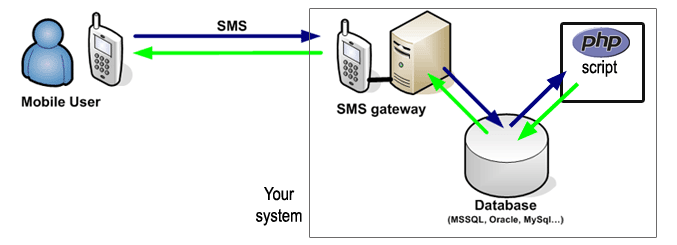
\includegraphics[width=\linewidth,height=\textheight,keepaspectratio]{SMS}

\hypersetup{
  pdfauthor={Athanasios Garyfalos},
  pdftitle={Django Rest Framework Sample of Work},
  pdfsubject={Guide Book for the Project},
  pdfkeywords={Key} {Words} {List},
  urlcolor=blue,
}

\title[SMS Service] % (optional, only for long titles)
{An SMS service to inform users when to depart from their location}
\subtitle{Train Karlskrona to Ronneby and Vise Versa}
\vspace*{-1.5em}
\author[Garyfalos, Bunyakitanon, Peng, Mazaheri]% (optional, for multiple authors)
{A.~Garyfalos \and M.~Bunyakitanon \and I.~Peng \and S.~Mazaheri}
\institute[Blekinge Tekniska Högskola, Karlskrona. Sweden] % (optional)
{
\\
\medskip
{
\emph{A.atga12@student.bth.se}
\emph{B.ltbu12@student.bth.se}
\emph{C.mepe12@student.bth.se}
\emph{D.shma12@student.bth.se}
}
}
\date[BTH 2013]{Presentation: 1, 2013}
\subject{Department of Computer Science}

\begin{document}

\begin{frame}[noframenumbering]
  \begin{center}
    % Upper part of the page
    %\vspace*{3.0em}
    
\includegraphics[width=0.15\textwidth]{BTH_logo}\\ [0.3cm]    

    \emph{Supervisor:} \\  
    Dr.~Fridensköld\\
    \textsc{Torbjörn} 
  \end{center}
  \titlepage
\end{frame}

\section*{Acknowledgements}
  \begin{frame}
    \begin{center}
{\footnotesize Acknowledgement: This work was performed within the Department of Computer Science (ET1208) project, which is supported by the Electrical and computer Sciences Engineering department. This is not an individual work we as SNMP group combined our expertise field and produce this work.}
    \end{center}
\end{frame}

\section*{Project Task}

\begin{frame}
\setbeamercovered{dynamic}%Makes the text appear before it presents nice!!!! 
\frametitle{Outline}
\tableofcontents[pausesections]
\end{frame}

\section{Project Description}
  \subsection{User Friendly}

\begin{frame}{Project Description}
\setbeamercovered{dynamic}%Makes the text appear before it presents nice!!!! 
    \begin{columns}[t] % contents are top vertically aligned
      \begin{column}[T]{5cm} % each column can also be its own environment
        \begin{itemize}
            \item<+-| alert@+> PDA, Smart Phone etc.
            \item<+-| alert@+> Enter data to webpage
            \item<+-| alert@+> Stored in Database
            \item<+-| alert@+> Calculations in the background will occur
            \item<+-| alert@+> Confirmation will be send to the user!
            \item<+-| alert@+> Done! Simple!
          \end{itemize}  
      \end{column}
    \begin{column}[T]{5cm} % alternative top-align that's better for graphics
      \begin{figure}
        \centerline{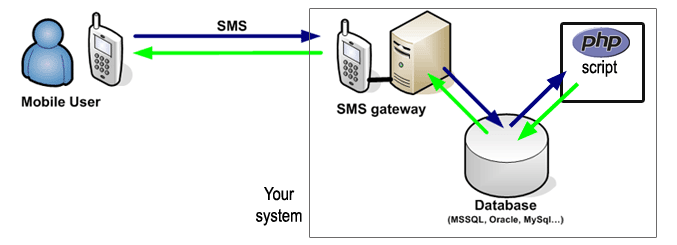
\includegraphics[scale=0.28]{SMS}}
        \vspace*{10pt}
        \captionsetup{justification=centering} %Center a two line caption
        \caption{Send / Receive SMS from PHP using a MySQL database}%~\cite{SMS}
        %\includegraphics[options]{path_to_image}syntax
      \end{figure}
    \end{column}
  \end{columns}
\end{frame}

  \subsection{Group members positions and responsibilities}

\begin{frame}
\setbeamercovered{dynamic}%Makes the text appear before it presents nice!!!! 
  \begin{exampleblock}{SNMP group members}
    \begin{itemize}
      \item Positions
      \item<1-| alert@1>> Athanasios Garyfalos (\alert{Project Manager})
      \item<2-| alert@2>> Monchai Bunyakitanon (\alert{Research and Development RnD})
      \item<3-| alert@3>> Iris Peng (\alert{Software Engineering})
      \item<4-| alert@4>> Shima Mazaheri (\alert{Test Engineering})
      \item Responsibilities
      \item<1-| alert@1>> Planning-execute-closing the project based on deadlines.
      \item<2-| alert@2>> Develop new ideas and products. Will give us the competitive edge.
      \item<3-| alert@3>> Develop and implement the ideas of the RnD.
      \item<4-| alert@4>> Test SW for Verification and validation.
    \end{itemize}
  \end{exampleblock}
\end{frame}

\subsection{Website ready and operating}

%\begin{frame}
%\setbeamercovered{dynamic} % Makes the text appear before it presents nice!!!! 
%  \begin{figure}
%  \vspace*{-130pt}
%    \makebox[\linewidth]{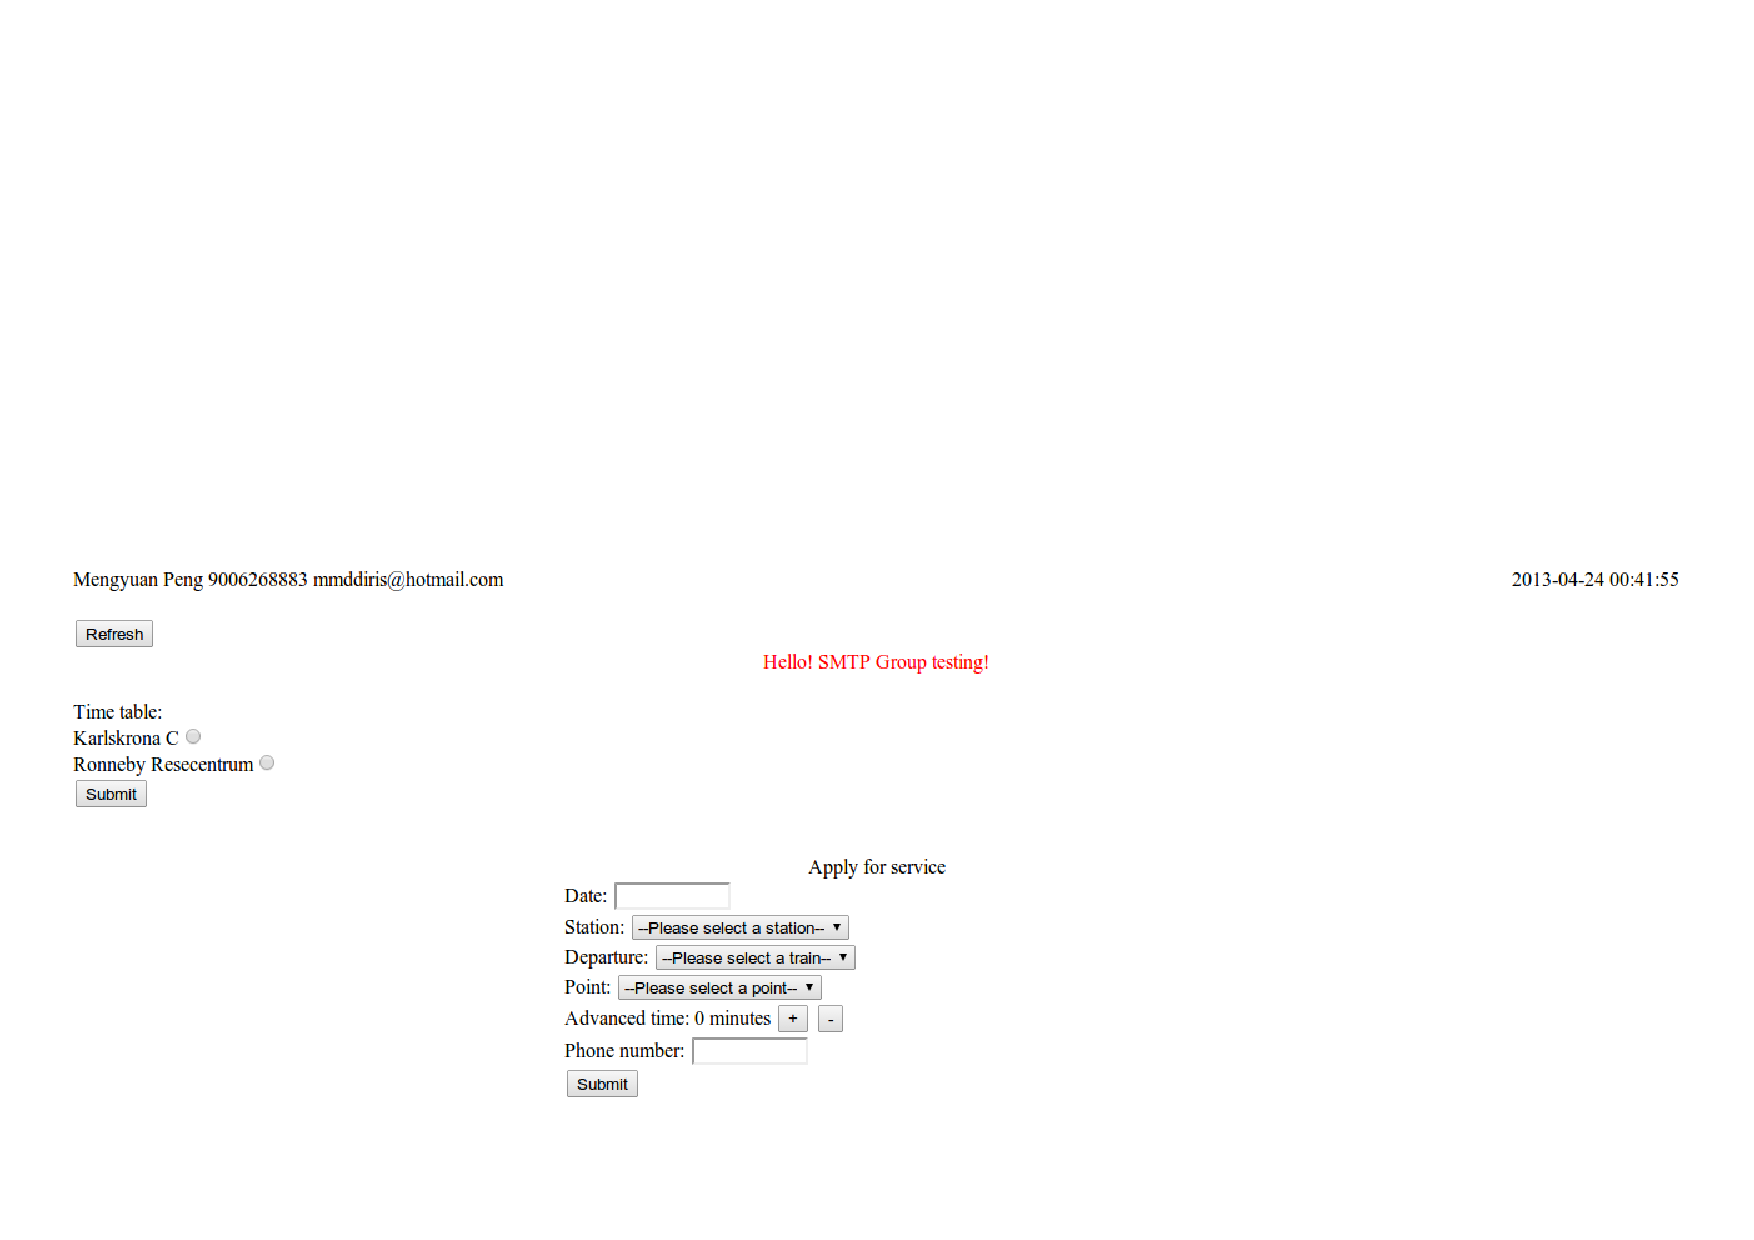
\includegraphics[pages=-,
%      [width=\paperwidth,
%       height=\paperheight,
%       keepaspectratio]{work}}
%      \caption{Web Server up and operating\label{fig:web}}
%        \begin{itemize}[<+->]
%          \pause
            %\item \url{http:80.78.219.77/SMTPGroup/main/test.php}
          %<+-| alert@+> 
%        \end{itemize}
%  \end{figure}
%\end{frame}

\begin{frame}{Project Analysis}
\setbeamercovered{dynamic}%Makes the text appear before it presents nice!!!! 
    \begin{columns}[t] % contents are top vertically aligned
      \begin{column}[T]{5cm} % each column can also be its own environment
        \begin{itemize}
            \item<+-| alert@+> Train departure station
            \item<+-| alert@+> Departure time
            \item<+-| alert@+> Users current location
            \item<+-| alert@+> Time interval
            \item<+-| alert@+> Inserting valid number
            \item<+-| alert@+> Walking distance calculation
            \item<+-| alert@+> 5.0 kilometers (km/h) %~\cite{wiki}
          \end{itemize}  
      \end{column}
    \begin{column}[T]{5cm} % alternative top-align that's better for graphics
      \begin{figure}
        \centerline{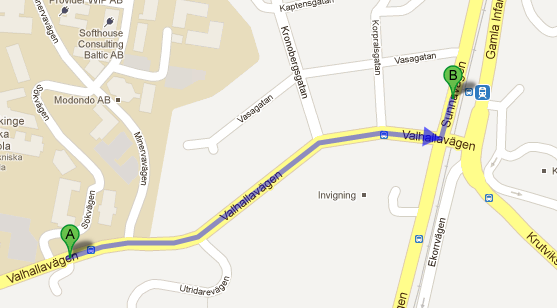
\includegraphics[scale=0.33]{path}}
        \vspace*{10pt}
        \captionsetup{justification=centering} %Center a two line caption
        \caption{From BTH to Bergåsa station}
        %\includegraphics[options]{path_to_image}syntax
      \end{figure}
    \end{column}
  \end{columns}
\end{frame}

%\section{}
\subsection{Integration Strategy}

%\begin{frame}{Integration Strategy}
%  \setbeamercovered{dynamic}
%    \begin{columns}[t] % contents are top vertically aligned
     %\column{.5\textwidth}
%      \begin{column}[T]{5cm} % each column can also be its own environment
%        \begin{itemize}[<+->]
%            \item WBS %~\cite{SNMP}
%            \item Start with low-level system
%            \item Integrate bottom-up
%            \item We continue until the system is created
%            \item Why ?
%        \end{itemize}  
%      \end{column}
%    \begin{column}[T]{5cm} % alternative top-align that's better for graphics
%      \begin{figure}
%        \vspace*{-140pt}
%          \makebox[\linewidth]{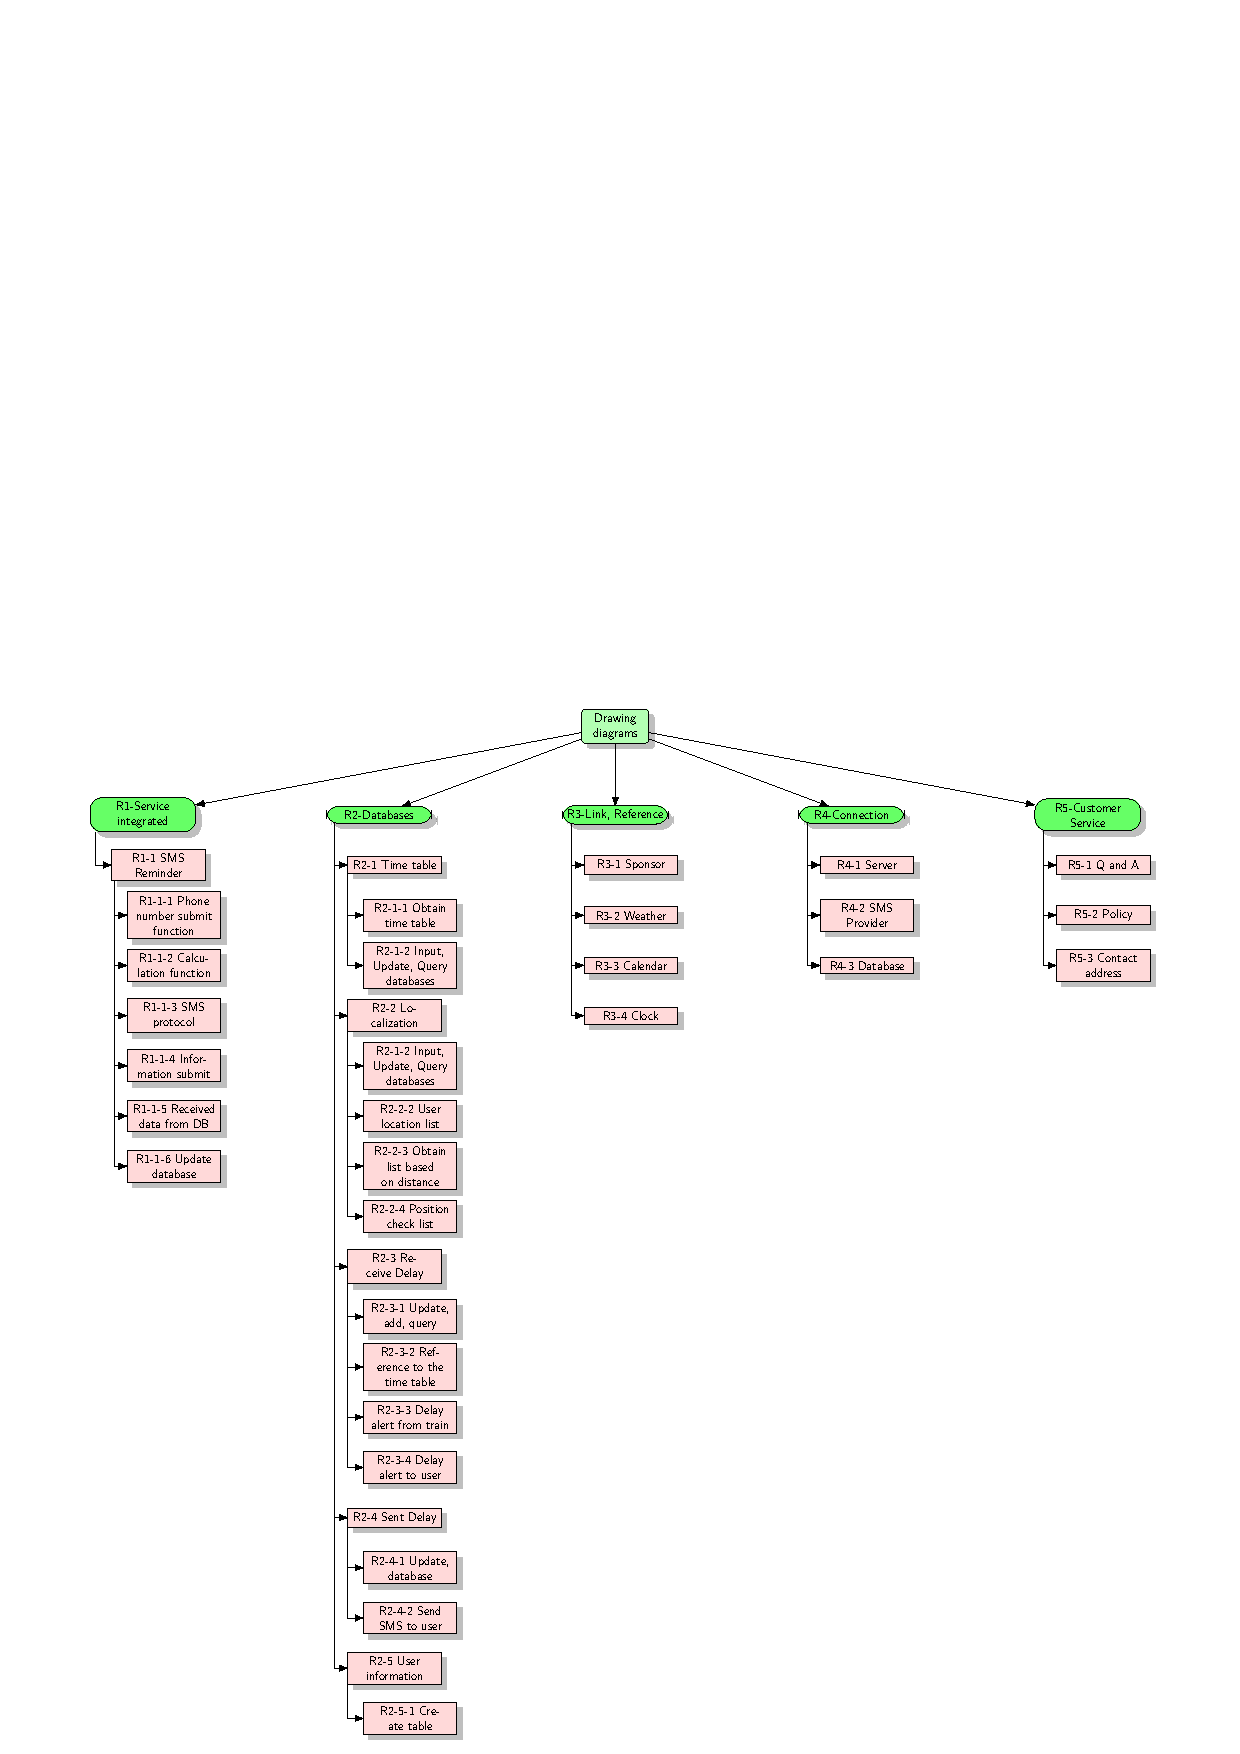
\includegraphics[pages=-,
%          [width=\paperwidth,
%           height=\paperheight,
%           keepaspectratio]{WBS}} %Include pdf picture in presentation
%        \captionsetup{justification=centering} %Center a two line caption
%        \caption{Work Breakdown Structure\label{fig:wbs}}
        %\includegraphics[options]{path_to_image}syntax
%      \end{figure}
%    \end{column}
%  \end{columns}
%\end{frame}

\section{Time allocation}
  \subsection{Time plan for whole project}
  
%\begin{frame}
%\setbeamercovered{dynamic}%Makes the text appear before it presents nice!!!! 
%  \begin{figure}
%  \vspace*{-115pt}
%    \makebox[\linewidth]{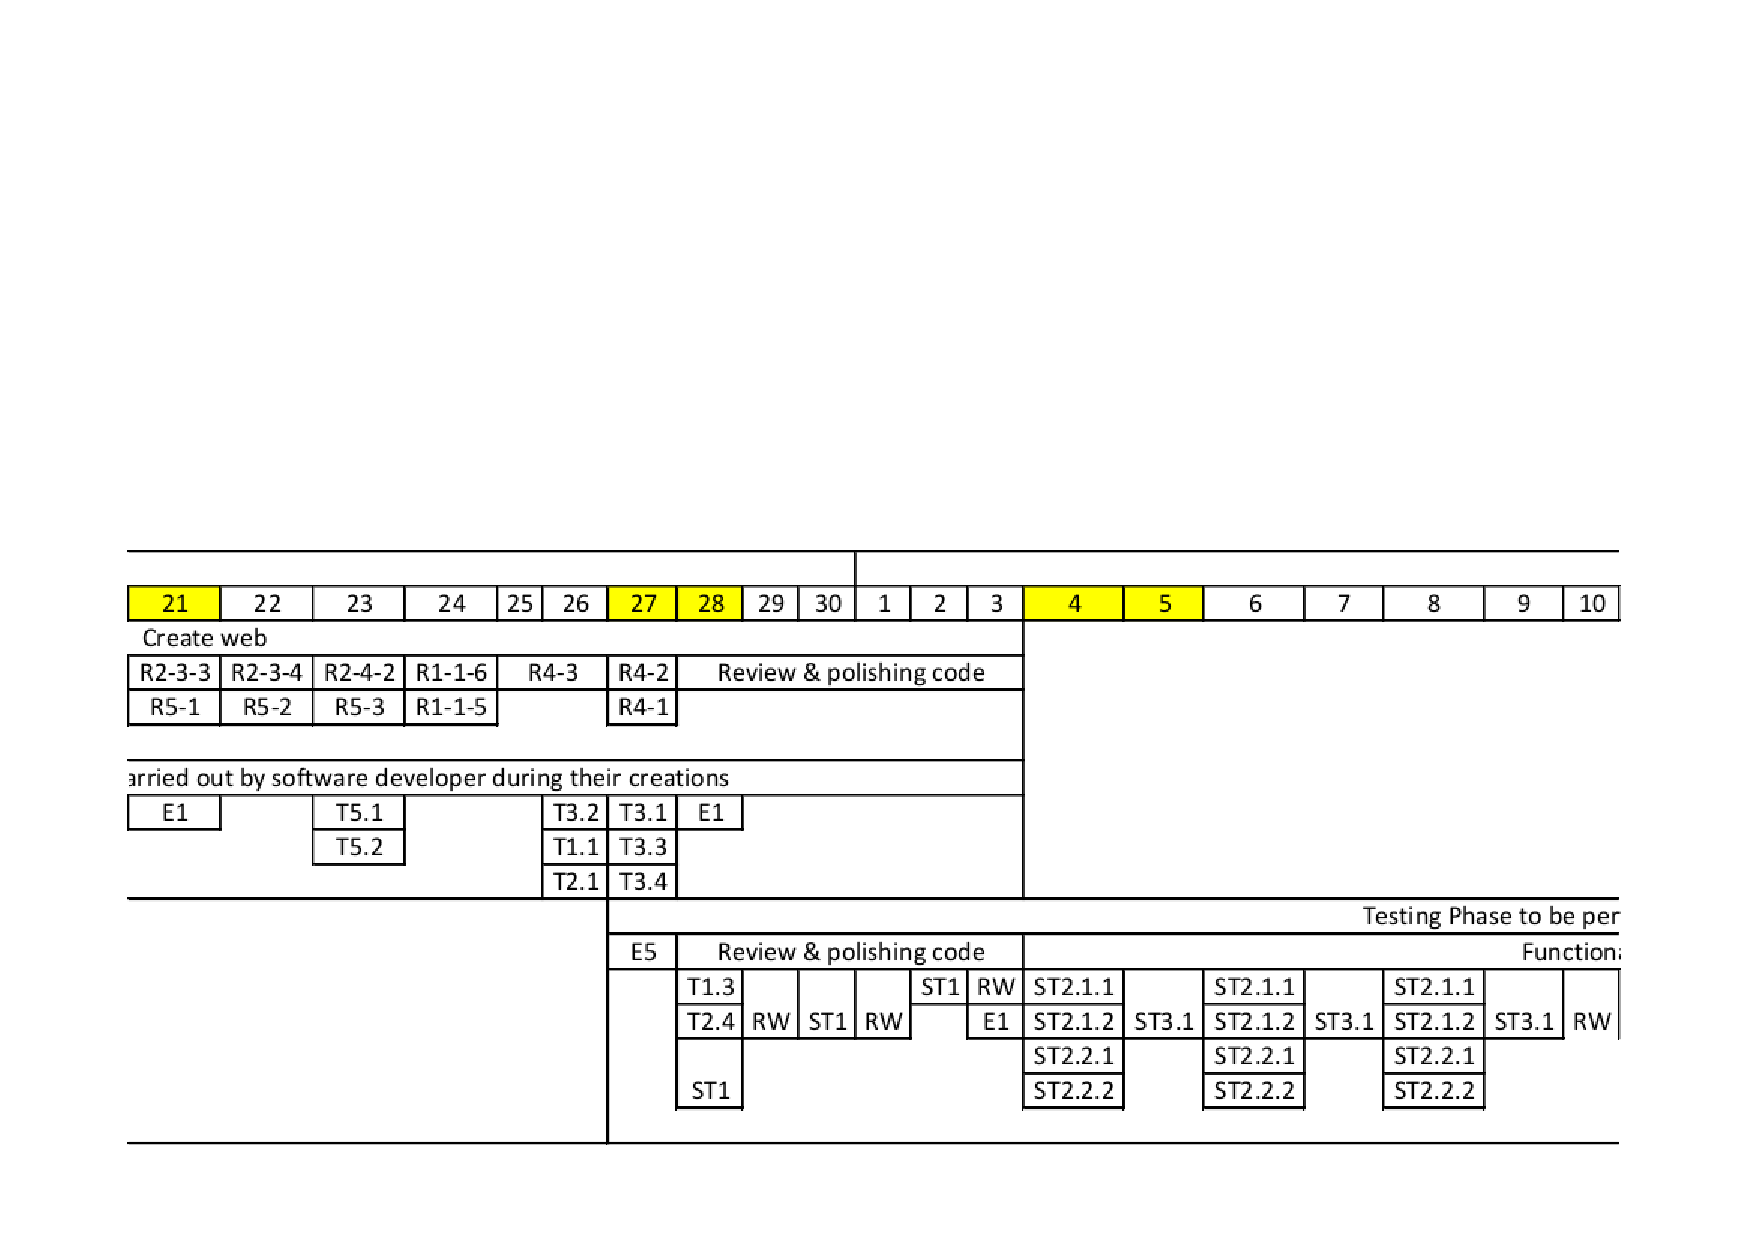
\includegraphics[pages=-,
%                                          [width=\paperwidth,
%                                           height=\paperheight,
%                                           keepaspectratio]{time}}
%      \caption{One part of the whole project Time Plan \label{fig:time}}
%        \begin{itemize}
%	        \pause
%          	\item Sample time plan for milestone: 2-3 
%          %<+-| alert@+> 
%        \end{itemize}
%  \end{figure}
%\end{frame}

  \subsection{Weekly projects}
\makeatletter %Step by step to show the table (all three lines) (1)
\let\slideno\beamer@slideinframe % (2)
\makeatother %(3)

\begin{frame}[t]
\rowcolors{1}{RoyalBlue!20}{RoyalBlue!5}
\onslide<2> {}
\onslide<3> {}

  \begin{table}
    \caption{Project Tracker Week: 3\label{tab:weekslu}}
    {\footnotesize
      \begin{tabular}{|>{\centering\arraybackslash}m{1.5cm}|>{\centering\arraybackslash}m{2.5cm}|>{\centering\arraybackslash}m{2.5cm}|>{\centering\arraybackslash}m{2.5cm}|}
\hline
\multicolumn{4}{| c |}{{\textbf{Slugging work}}} \\
 \hline
\textbf{ID} & \textbf{Completion (\%)} & \textbf{Time spend (hours)} & \textbf{Estimated time left (hours)} \\
\hline
\ifnum\slideno>1 
  R1-1-3 & 0 & 0 & 4 \\
  R2-2-1 & 70 & 3 & 1 \\
  R2-2-4 & 70 & 3 & 1 \\
  R2-3-3 & 20 & 7 & 3 \\
  R2-4-1 & 0 & 0 & 4 \\
  R3-3 & 50 & 2 & 2 \\
  R5-1 & 0 & 4 & 4 \\
  \hline
  \ifnum\slideno>2
  \multicolumn{2}{|c|}{\textbf{Total:}} & 19 & 19\\ \hline
  
\fi\fi
    \end{tabular}
    }
  \end{table}
\end{frame}


\begin{frame}[t]
\setbeamercovered{dynamic}%Makes the text appear before it presents nice!!!! 
\rowcolors{1}{RoyalBlue!20}{RoyalBlue!5}
\onslide<2> {}
\onslide<3-> {}

  \begin{table}
    \caption{Advanced Project Tracker Week: 3\label{tab:weekadv}}
    {\footnotesize
   \begin{tabular}{|>{\centering\arraybackslash}m{1.5cm}|>{\centering\arraybackslash}m{2.5cm}|>{\centering\arraybackslash}m{2.5cm}|>{\centering\arraybackslash}m{2.5cm}|}
\hline
  
  \multicolumn{4}{|c|}{\textbf{Work in advance}} \\
  \hline
  \textbf{ID} & \textbf{Completion (\%)} & \textbf{Time spend (hours)} & \textbf{Estimated time left (hours)} \\
  \hline
  \ifnum\slideno>1
  R5.3 & 100 & 4 & 0 \\
  R4.3 & 50 & 4 & 4 \\
  R4.1 & 100 & 4 & 0 \\
  \hline
  \ifnum\slideno>2
  \multicolumn{2}{|c|}{\textbf{Total:}} & 12 & 23\\ \hline
  \fi\fi
    \end{tabular}
    }
  \end{table}

    \begin{itemize}[<+->]
      \item<4-> As a final step we make the summation of working hours \alert{left} from both parts and change the \alert{goals of the project!}
      \item<5-> We check weekly to see how many \alert{extra features} we can add based on \alert{time!}
      \item<6-> Program changes \alert{weekly}, due to some projects require more time \alert{than estimated} and vise versa some require \alert{less} time!
    \end{itemize}
\end{frame}

\subsection{Next Actions and Problems}

\begin{frame}{Next Actions \& Problems}
  \setbeamercovered{dynamic}
    \begin{columns}
      \column{.5\textwidth}
        \begin{block}{Next Actions}
          \begin{enumerate}
            \item Complete coding \\ \pause
            \item Start testing procedure \\ \pause
            \item Meet acceptance criteria \\ \pause
            \item Complete project on time \\ \pause
            %\item Why ? \\ \pause
          \end{enumerate} 
        \end{block}
      \column{.5\textwidth}
        \begin{block}{Problems faced}
          \begin{enumerate}
            \item No \alert{API} available for testing \\ \pause
            \item We do not have a real server \\ \pause
            \item New programming languages \\ \pause
            \item No sponsor / no funding  \\ \pause
            %\item Why ?
          \end{enumerate}         
        \end{block}
    \end{columns}
    \begin{block}{Actions against problems}
      \begin{itemize}
        \item Print the information send by the database to the Terminal \\ \pause
        \item We will use our own computer as server for testing purposes \\ \pause
        \item Become familiar with the programming languages A.S.A.P \\ \pause
        \item We are trying not to spend money procedure modifications
      \end{itemize}
    \end{block}
\end{frame}

\subsection{Quality Measures}
\setbeamercovered{dynamic}
\begin{frame}
  \begin{exampleblock}{Quality measures that we have and we implement}
    \begin{itemize}[<+->]
      \item Time plan that we follow and modify step by step\\
       \textcolor{magenta}{(\emph{{See figure:~\ref{fig:time}~\nameref{fig:time}}})}
      \item Acceptance criteria
      \item Documentation analysis
      \item Target meet deliveries so far at least
      \item Code / debugging tools
    \end{itemize}
  \end{exampleblock}
\end{frame}

\section{Summary}
  \subsection{Key points repetition}
  
\begin{frame}
\setbeamercovered{dynamic}
  \begin{exampleblock}{Summary}
    \begin{itemize}[<+->]
      \item Project Description
      \item Integration Strategy
      \item Project Time Plan
      \item Actions and Problems
      \item Quality Measures \\ \pause
    \end{itemize}
  \end{exampleblock}
  \begin{exampleblock}{Extra Notes}
    \begin{itemize}[<+->]
      \item Both the Report and the Presentation where written in \LaTeX
      \item Many people ask \alert{Why spend so much time!!!}
      \item \alert{Answer:} The output quality is above expectations!
    \end{itemize}
  \end{exampleblock}
\end{frame}

\subsection*{Questions}
\begin{frame}
%\begin{overlayarea}{\textwidth}{3cm}
    %\only<1>{Some text for the first slide.\\Possibly several lines long.}
    %\only<2>{Replacement on the second slide.}
%\end{overlayarea}
  \begin{itemize}
     \Large
    \item \colorbox{yellow}{Thanks a lot – questions \& comments?}
  \end{itemize} 
\end{frame}

\section{Bibliography}
  \subsection*{Web and Articles}

\begin{frame}[allowframebreaks]
  \frametitle<presentation>{References}
  \bibliographystyle{amsalpha}   
  \begin{thebibliography}{10}
  \setbeamertemplate{bibliography item}[online]
  \bibitem{SMS}
  Ozeki Informatics Ltd.
    \newblock {\emph{Proof of the Riemann Hypothesis}}
    \newblock preprint (2003)
    \newblock available at \url{http://www.math.drofnats.edu/riemann.ps}.
  \setbeamertemplate{bibliography item}[online]
  \bibitem{wiki}
  From Wikipedia, the free encyclopedia
    \newblock {\emph{Walking}}
    \newblock preprint (2013)
    \newblock available at \url{https://en.wikipedia.org/wiki/Walking}.
  \setbeamertemplate{bibliography item}[article]
  \bibitem{SNMP}
    A.~Garyfalos \& M.~Bunyakitanon \& M.~Peng \& S.~Mazaheri.
    \newblock Volume: 3, Produced in \LaTeX
    \newblock {\emph{Blekinge Tekniska Högskola}}
  \end{thebibliography}
\end{frame}

\end{document}
